% Wheeled Humanoid - wiring diagram, standalone bench copy. pdflatex wiring.tex
\documentclass[10pt,a4paper]{article}
\usepackage[T1]{fontenc}\usepackage[utf8]{inputenc}
\usepackage[scaled=0.95]{helvet}\renewcommand{\familydefault}{\sfdefault}
\usepackage[a4paper,margin=18mm,top=20mm,bottom=20mm]{geometry}
\usepackage{graphicx,xcolor,booktabs,tabularx,longtable,array,float,enumitem,textcomp,amsmath,titlesec,fancyhdr}
\usepackage{tikz}
\definecolor{rasred}{gray}{0}\definecolor{raspurple}{gray}{0}\definecolor{soft}{gray}{0.95}
\definecolor{pwr}{HTML}{C0392B}\definecolor{sig}{HTML}{2C6FBB}\definecolor{sda}{HTML}{1E8E4E}\definecolor{scl}{HTML}{D9820B}\definecolor{act}{HTML}{E08E0B}
\newcolumntype{L}{>{\raggedright\arraybackslash}X}\newcolumntype{P}[1]{>{\raggedright\arraybackslash}p{#1}}
\titleformat{\section}{\Large\bfseries\color{rasred}}{}{0em}{}
\titleformat{\subsubsection}{\normalsize\bfseries\color{raspurple}}{}{0em}{}
\setlist{nosep,leftmargin=1.4em}\setlength{\parindent}{0pt}\setlength{\parskip}{5pt}\renewcommand{\arraystretch}{1.15}
\pagestyle{fancy}\fancyhf{}\lhead{\small\color{gray}Wheeled Humanoid \textperiodcentered{} Wiring diagram}\rhead{\small\color{gray}Sheet \thepage}\renewcommand{\headrulewidth}{0.3pt}
\begin{document}
\section{Sheet 1: power wiring}
Every terminal from the battery to each load. Thick lines are 14 AWG, thin lines 16 AWG.
\begin{center}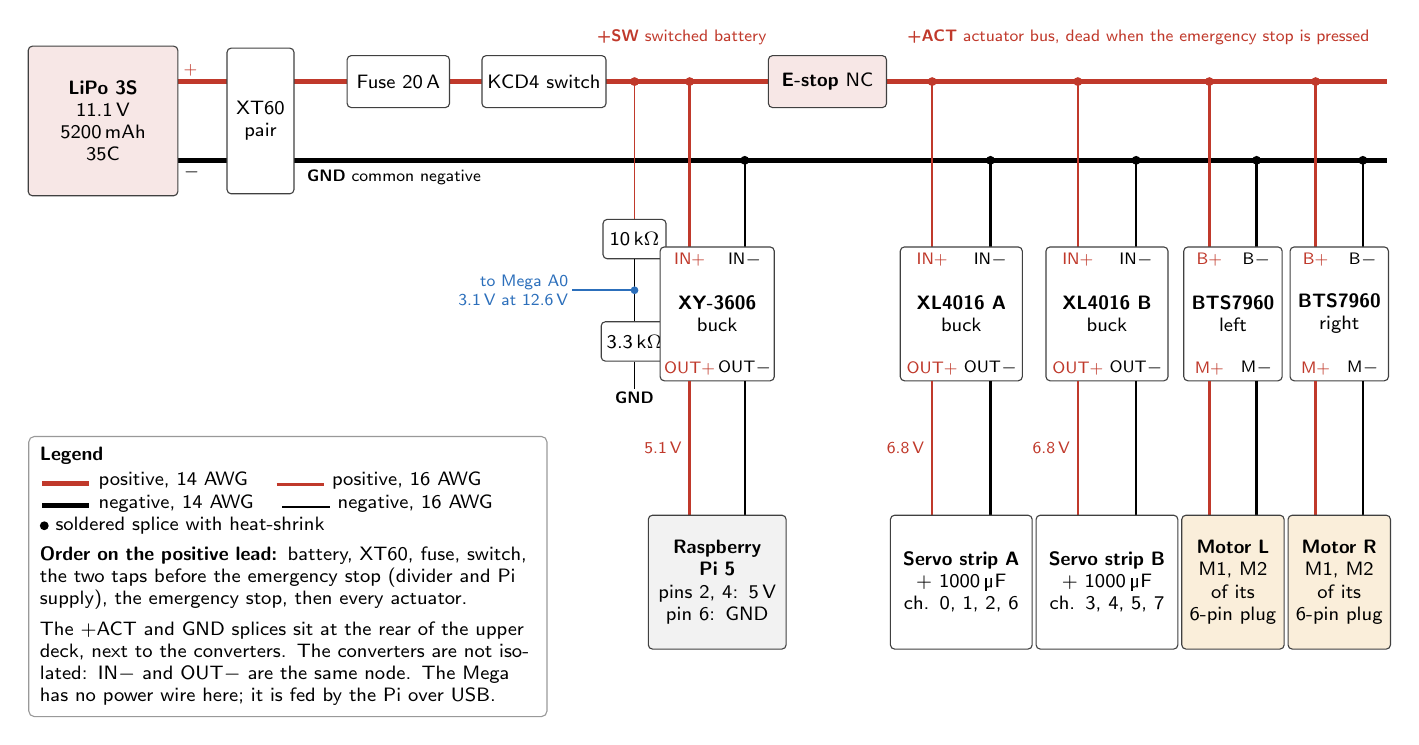
\begin{tikzpicture}[font=\scriptsize, cmp/.style={draw=black!75,rounded corners=1.5pt,fill=white,align=center,inner sep=2pt}, p/.style={draw=pwr}, n/.style={draw=black}, t/.style={font=\fontsize{6}{7}\selectfont,inner sep=1pt}]
\draw[p,line width=1.7pt] (1.9,0) -- (17.25,0);
\draw[n,line width=1.7pt] (1.9,-1.0) -- (17.25,-1.0);
\node[cmp,fill=pwr!12,minimum width=1.9cm,minimum height=1.9cm] at (0.95,-0.5) {\textbf{LiPo 3S}\\11.1\,V\\5200\,mAh\\35C};
\node[t,anchor=south west,text=pwr] at (1.93,0.03) {+}; \node[t,anchor=north west] at (1.93,-1.03) {$-$};
\node[cmp,minimum width=0.85cm,minimum height=1.85cm] at (2.95,-0.5) {XT60\\pair};
\node[cmp,minimum width=1.3cm,minimum height=0.66cm] at (4.7,0) {Fuse 20\,A};
\node[cmp,minimum width=1.4cm,minimum height=0.66cm] at (6.55,0) {KCD4 switch};
\node[cmp,fill=pwr!12,minimum width=1.5cm,minimum height=0.66cm] at (10.15,0) {\textbf{E-stop} NC};
\node[t,text=pwr,anchor=south] at (8.3,0.42) {\textbf{+SW} switched battery}; \node[t,text=pwr,anchor=south] at (14.1,0.42) {\textbf{+ACT} actuator bus, dead when the emergency stop is pressed};
\node[t,anchor=north west] at (3.5,-1.08) {\textbf{GND} common negative};
\fill[pwr] (7.7,0) circle (1.6pt); \draw[p,line width=0.5pt] (7.7,0) -- (7.7,-1.75);
\node[cmp,minimum width=0.8cm,minimum height=0.5cm] (r1) at (7.7,-2.0) {10\,k$\Omega$};
\node[cmp,minimum width=0.8cm,minimum height=0.5cm] (r2) at (7.7,-3.3) {3.3\,k$\Omega$};
\draw[line width=0.5pt] (r1) -- (r2); \fill[sig] (7.7,-2.65) circle (1.4pt); \draw[draw=sig,line width=0.6pt] (7.7,-2.65) -- (6.9,-2.65); \node[t,text=sig,anchor=east,align=right] at (6.9,-2.65) {to Mega A0\\3.1\,V at 12.6\,V};
\draw[n,line width=0.5pt] (r2) -- (7.7,-3.9); \node[t,anchor=north] at (7.7,-3.9) {\textbf{GND}};
\fill[pwr] (8.4,0) circle (1.6pt); \draw[p,line width=0.9pt] (8.4,0) -- (8.4,-2.1);
\fill (9.1,-1.0) circle (1.6pt); \draw[n,line width=0.9pt] (9.1,-1.0) -- (9.1,-2.1);
\node[cmp,fill=white,minimum width=1.45cm,minimum height=1.7cm] at (8.75,-2.95) {\textbf{XY-3606}\\buck};
\node[t,anchor=north,text=pwr] at (8.4,-2.13) {IN+}; \node[t,anchor=north] at (9.1,-2.13) {IN$-$};
\node[t,anchor=south,text=pwr] at (8.4,-3.77) {OUT+}; \node[t,anchor=south] at (9.1,-3.77) {OUT$-$};
\draw[p,line width=0.9pt] (8.4,-3.8) -- (8.4,-5.5); \draw[n,line width=0.9pt] (9.1,-3.8) -- (9.1,-5.5);
\node[cmp,fill=soft,minimum width=1.75cm,minimum height=1.7cm,anchor=north,text width=1.6cm] at (8.75,-5.5) {\textbf{Raspberry Pi 5}\\pins 2, 4: 5\,V\\pin 6: GND};
\node[t,anchor=east,text=pwr,align=right] at (8.34,-4.65) {5.1\,V};
\fill[pwr] (11.48,0) circle (1.6pt); \draw[p,line width=0.9pt] (11.48,0) -- (11.48,-2.1);
\fill (12.22,-1.0) circle (1.6pt); \draw[n,line width=0.9pt] (12.22,-1.0) -- (12.22,-2.1);
\node[cmp,fill=white,minimum width=1.55cm,minimum height=1.7cm] at (11.85,-2.95) {\textbf{XL4016 A}\\buck};
\node[t,anchor=north,text=pwr] at (11.48,-2.13) {IN+}; \node[t,anchor=north] at (12.22,-2.13) {IN$-$};
\node[t,anchor=south,text=pwr] at (11.48,-3.77) {OUT+}; \node[t,anchor=south] at (12.22,-3.77) {OUT$-$};
\draw[p,line width=0.9pt] (11.48,-3.8) -- (11.48,-5.5); \draw[n,line width=0.9pt] (12.22,-3.8) -- (12.22,-5.5);
\node[cmp,fill=white,minimum width=1.8cm,minimum height=1.7cm,anchor=north,text width=1.6500000000000001cm] at (11.85,-5.5) {\textbf{Servo strip A}\\+ 1000\,\textmu F\\ch. 0, 1, 2, 6};
\node[t,anchor=east,text=pwr,align=right] at (11.42,-4.65) {6.8\,V};
\fill[pwr] (13.33,0) circle (1.6pt); \draw[p,line width=0.9pt] (13.33,0) -- (13.33,-2.1);
\fill (14.07,-1.0) circle (1.6pt); \draw[n,line width=0.9pt] (14.07,-1.0) -- (14.07,-2.1);
\node[cmp,fill=white,minimum width=1.55cm,minimum height=1.7cm] at (13.7,-2.95) {\textbf{XL4016 B}\\buck};
\node[t,anchor=north,text=pwr] at (13.33,-2.13) {IN+}; \node[t,anchor=north] at (14.07,-2.13) {IN$-$};
\node[t,anchor=south,text=pwr] at (13.33,-3.77) {OUT+}; \node[t,anchor=south] at (14.07,-3.77) {OUT$-$};
\draw[p,line width=0.9pt] (13.33,-3.8) -- (13.33,-5.5); \draw[n,line width=0.9pt] (14.07,-3.8) -- (14.07,-5.5);
\node[cmp,fill=white,minimum width=1.8cm,minimum height=1.7cm,anchor=north,text width=1.6500000000000001cm] at (13.7,-5.5) {\textbf{Servo strip B}\\+ 1000\,\textmu F\\ch. 3, 4, 5, 7};
\node[t,anchor=east,text=pwr,align=right] at (13.27,-4.65) {6.8\,V};
\fill[pwr] (15.0,0) circle (1.6pt); \draw[p,line width=0.9pt] (15.0,0) -- (15.0,-2.1);
\fill (15.6,-1.0) circle (1.6pt); \draw[n,line width=0.9pt] (15.6,-1.0) -- (15.6,-2.1);
\node[cmp,fill=white,minimum width=1.25cm,minimum height=1.7cm] at (15.3,-2.95) {\textbf{BTS7960}\\left};
\node[t,anchor=north,text=pwr] at (15.0,-2.13) {B+}; \node[t,anchor=north] at (15.6,-2.13) {B$-$};
\node[t,anchor=south,text=pwr] at (15.0,-3.77) {M+}; \node[t,anchor=south] at (15.6,-3.77) {M$-$};
\draw[p,line width=0.9pt] (15.0,-3.8) -- (15.0,-5.5); \draw[n,line width=0.9pt] (15.6,-3.8) -- (15.6,-5.5);
\node[cmp,fill=act!15,minimum width=1.3cm,minimum height=1.7cm,anchor=north,text width=1.1500000000000001cm] at (15.3,-5.5) {\textbf{Motor L}\\M1, M2 of its 6-pin plug};
\fill[pwr] (16.35,0) circle (1.6pt); \draw[p,line width=0.9pt] (16.35,0) -- (16.35,-2.1);
\fill (16.95,-1.0) circle (1.6pt); \draw[n,line width=0.9pt] (16.95,-1.0) -- (16.95,-2.1);
\node[cmp,fill=white,minimum width=1.25cm,minimum height=1.7cm] at (16.65,-2.95) {\textbf{BTS7960}\\right};
\node[t,anchor=north,text=pwr] at (16.35,-2.13) {B+}; \node[t,anchor=north] at (16.95,-2.13) {B$-$};
\node[t,anchor=south,text=pwr] at (16.35,-3.77) {M+}; \node[t,anchor=south] at (16.95,-3.77) {M$-$};
\draw[p,line width=0.9pt] (16.35,-3.8) -- (16.35,-5.5); \draw[n,line width=0.9pt] (16.95,-3.8) -- (16.95,-5.5);
\node[cmp,fill=act!15,minimum width=1.3cm,minimum height=1.7cm,anchor=north,text width=1.1500000000000001cm] at (16.65,-5.5) {\textbf{Motor R}\\M1, M2 of its 6-pin plug};
\node[anchor=north west,align=left,font=\scriptsize,text width=6.3cm,draw=black!40,rounded corners=2pt,inner sep=4pt] at (0,-4.5) {\textbf{Legend}\\[1pt]\tikz{\draw[draw=pwr,line width=1.7pt] (0,0)--(0.6,0);} positive, 14 AWG \quad \tikz{\draw[draw=pwr,line width=0.9pt] (0,0)--(0.6,0);} positive, 16 AWG\\\tikz{\draw[line width=1.7pt] (0,0)--(0.6,0);} negative, 14 AWG \quad \tikz{\draw[line width=0.9pt] (0,0)--(0.6,0);} negative, 16 AWG\\\tikz{\fill (0,0) circle (1.6pt);} soldered splice with heat-shrink\\[3pt]\textbf{Order on the positive lead:} battery, XT60, fuse, switch, the two taps before the emergency stop (divider and Pi supply), the emergency stop, then every actuator.\\[3pt]The +ACT and GND splices sit at the rear of the upper deck, next to the converters. The converters are not isolated: IN$-$ and OUT$-$ are the same node. The Mega has no power wire here; it is fed by the Pi over USB.};
\end{tikzpicture}\end{center}
\clearpage
\section{Sheet 2: signal wiring}
Every module pin to its controller pin. Blue: digital signal. Green: I\textsuperscript{2}C SDA. Orange: I\textsuperscript{2}C SCL. Red and black tags: 5\,V and GND from the Mega (3.3\,V and GND from the Pi for the OLEDs).
\begin{center}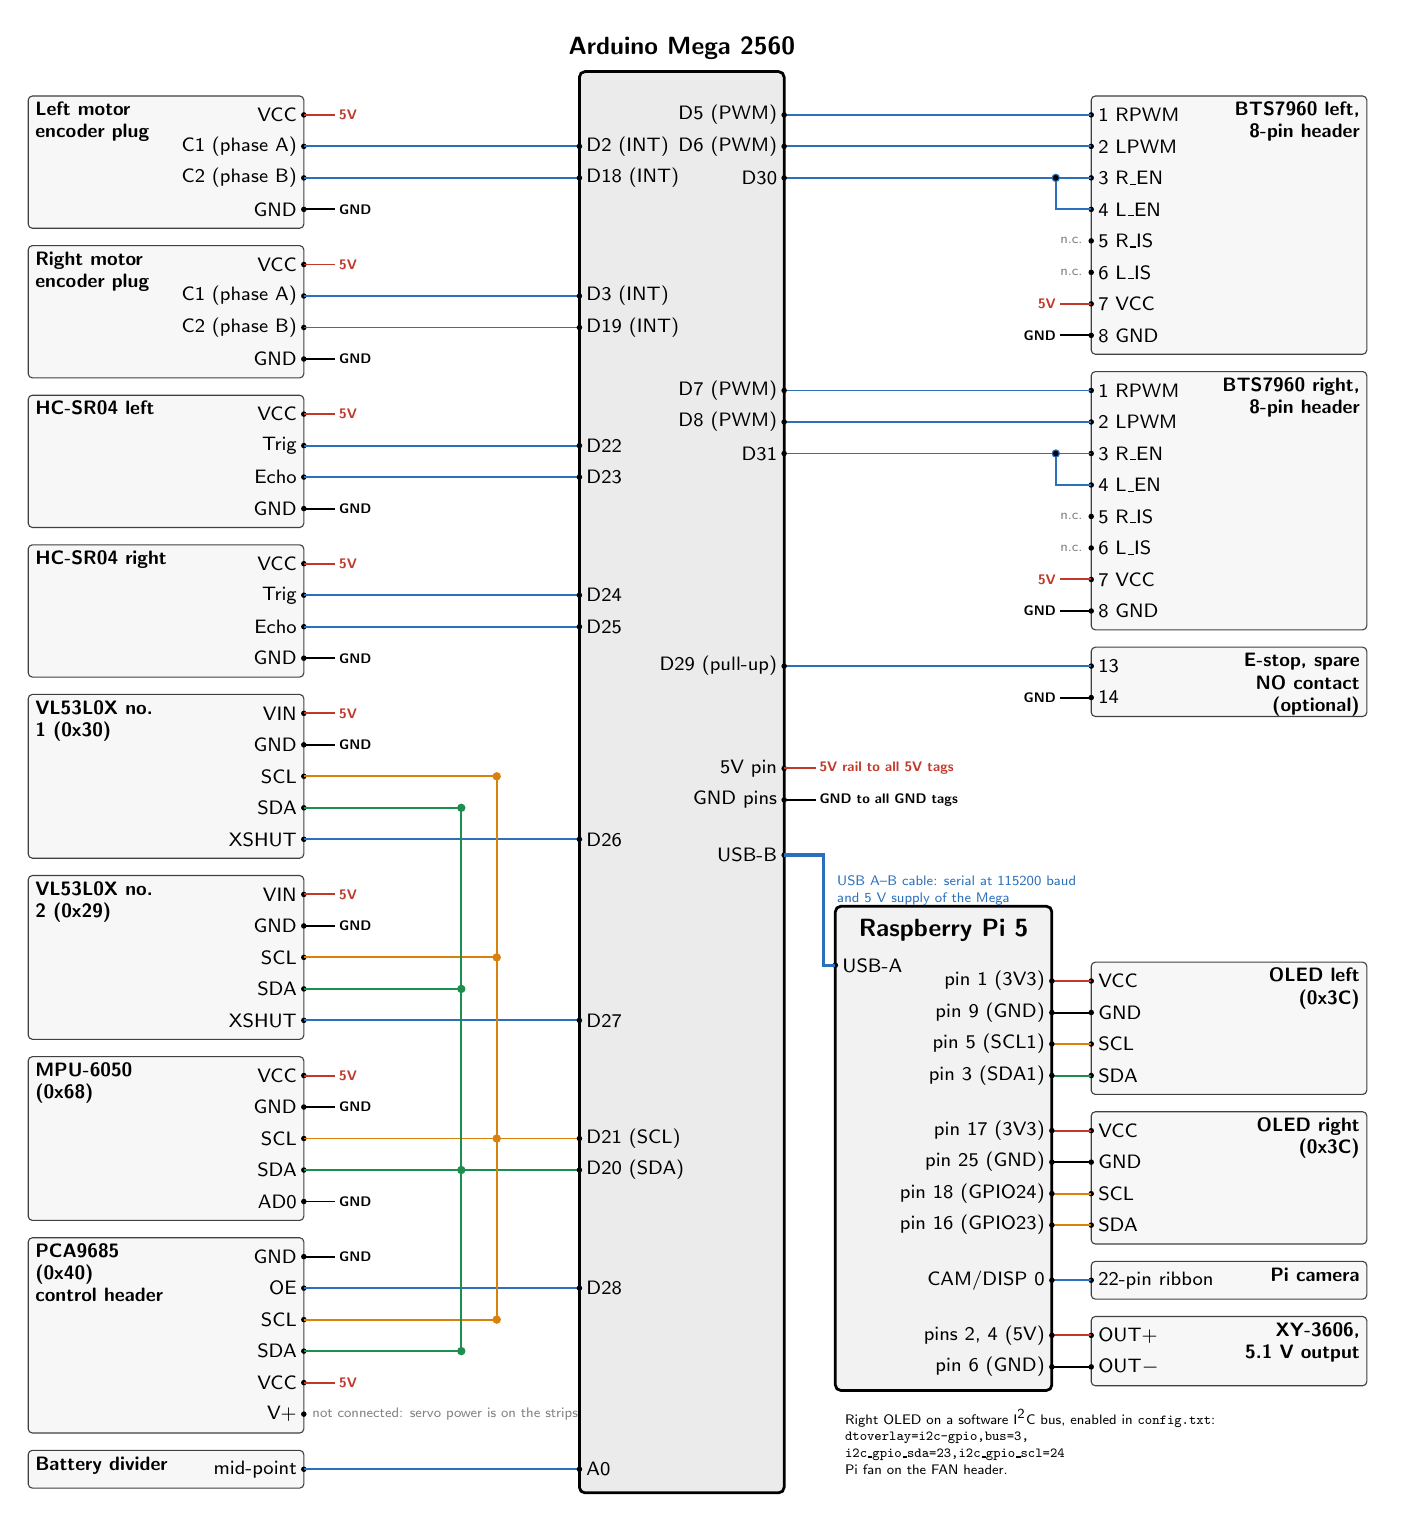
\begin{tikzpicture}[font=\scriptsize, mod/.style={draw=black!75,rounded corners=1.5pt,fill=black!3}, wire/.style={line width=0.7pt}, tag/.style={font=\tiny\bfseries,inner sep=1.2pt}, sig/.style={draw=sig,text=sig}, sda/.style={draw=sda,text=sda,fill=sda}, scl/.style={draw=scl,text=scl,fill=scl}, pwr/.style={draw=pwr}]
\draw[mod] (0.0,0.24) rectangle (3.5,-1.44);
\node[anchor=north west,align=left,text width=1.75cm,font=\scriptsize\bfseries,inner sep=1.5pt] at (0.03,0.22) {Left motor\\encoder plug};
\node[anchor=east,font=\scriptsize,inner sep=1.5pt] at (3.47,0.0) {VCC};
\fill (3.5,0.0) circle (1pt);
\draw[wire,pwr] (3.5,0.0) -- (3.9,0.0);
\node[tag,text=pwr,anchor=west] at (3.9,0.0) {5V};
\node[anchor=east,font=\scriptsize,inner sep=1.5pt] at (3.47,-0.4) {C1 (phase A)};
\fill (3.5,-0.4) circle (1pt);
\draw[wire,sig] (3.5,-0.4) -- (7.0,-0.4);
\node[anchor=east,font=\scriptsize,inner sep=1.5pt] at (3.47,-0.8) {C2 (phase B)};
\fill (3.5,-0.8) circle (1pt);
\draw[wire,sig] (3.5,-0.8) -- (7.0,-0.8);
\node[anchor=east,font=\scriptsize,inner sep=1.5pt] at (3.47,-1.2) {GND};
\fill (3.5,-1.2) circle (1pt);
\draw[wire,black] (3.5,-1.2) -- (3.9,-1.2);
\node[tag,,anchor=west] at (3.9,-1.2) {GND};
\draw[mod] (0.0,-1.66) rectangle (3.5,-3.34);
\node[anchor=north west,align=left,text width=1.75cm,font=\scriptsize\bfseries,inner sep=1.5pt] at (0.03,-1.68) {Right motor\\encoder plug};
\node[anchor=east,font=\scriptsize,inner sep=1.5pt] at (3.47,-1.9) {VCC};
\fill (3.5,-1.9) circle (1pt);
\draw[wire,pwr] (3.5,-1.9) -- (3.9,-1.9);
\node[tag,text=pwr,anchor=west] at (3.9,-1.9) {5V};
\node[anchor=east,font=\scriptsize,inner sep=1.5pt] at (3.47,-2.3) {C1 (phase A)};
\fill (3.5,-2.3) circle (1pt);
\draw[wire,sig] (3.5,-2.3) -- (7.0,-2.3);
\node[anchor=east,font=\scriptsize,inner sep=1.5pt] at (3.47,-2.7) {C2 (phase B)};
\fill (3.5,-2.7) circle (1pt);
\draw[wire,sig] (3.5,-2.7) -- (7.0,-2.7);
\node[anchor=east,font=\scriptsize,inner sep=1.5pt] at (3.47,-3.1) {GND};
\fill (3.5,-3.1) circle (1pt);
\draw[wire,black] (3.5,-3.1) -- (3.9,-3.1);
\node[tag,,anchor=west] at (3.9,-3.1) {GND};
\draw[mod] (0.0,-3.56) rectangle (3.5,-5.24);
\node[anchor=north west,align=left,text width=1.75cm,font=\scriptsize\bfseries,inner sep=1.5pt] at (0.03,-3.58) {HC-SR04 left};
\node[anchor=east,font=\scriptsize,inner sep=1.5pt] at (3.47,-3.8) {VCC};
\fill (3.5,-3.8) circle (1pt);
\draw[wire,pwr] (3.5,-3.8) -- (3.9,-3.8);
\node[tag,text=pwr,anchor=west] at (3.9,-3.8) {5V};
\node[anchor=east,font=\scriptsize,inner sep=1.5pt] at (3.47,-4.2) {Trig};
\fill (3.5,-4.2) circle (1pt);
\draw[wire,sig] (3.5,-4.2) -- (7.0,-4.2);
\node[anchor=east,font=\scriptsize,inner sep=1.5pt] at (3.47,-4.6) {Echo};
\fill (3.5,-4.6) circle (1pt);
\draw[wire,sig] (3.5,-4.6) -- (7.0,-4.6);
\node[anchor=east,font=\scriptsize,inner sep=1.5pt] at (3.47,-5.0) {GND};
\fill (3.5,-5.0) circle (1pt);
\draw[wire,black] (3.5,-5.0) -- (3.9,-5.0);
\node[tag,,anchor=west] at (3.9,-5.0) {GND};
\draw[mod] (0.0,-5.46) rectangle (3.5,-7.14);
\node[anchor=north west,align=left,text width=1.75cm,font=\scriptsize\bfseries,inner sep=1.5pt] at (0.03,-5.48) {HC-SR04 right};
\node[anchor=east,font=\scriptsize,inner sep=1.5pt] at (3.47,-5.7) {VCC};
\fill (3.5,-5.7) circle (1pt);
\draw[wire,pwr] (3.5,-5.7) -- (3.9,-5.7);
\node[tag,text=pwr,anchor=west] at (3.9,-5.7) {5V};
\node[anchor=east,font=\scriptsize,inner sep=1.5pt] at (3.47,-6.1) {Trig};
\fill (3.5,-6.1) circle (1pt);
\draw[wire,sig] (3.5,-6.1) -- (7.0,-6.1);
\node[anchor=east,font=\scriptsize,inner sep=1.5pt] at (3.47,-6.5) {Echo};
\fill (3.5,-6.5) circle (1pt);
\draw[wire,sig] (3.5,-6.5) -- (7.0,-6.5);
\node[anchor=east,font=\scriptsize,inner sep=1.5pt] at (3.47,-6.9) {GND};
\fill (3.5,-6.9) circle (1pt);
\draw[wire,black] (3.5,-6.9) -- (3.9,-6.9);
\node[tag,,anchor=west] at (3.9,-6.9) {GND};
\draw[mod] (0.0,-7.36) rectangle (3.5,-9.44);
\node[anchor=north west,align=left,text width=1.75cm,font=\scriptsize\bfseries,inner sep=1.5pt] at (0.03,-7.38) {VL53L0X no. 1 (0x30)};
\node[anchor=east,font=\scriptsize,inner sep=1.5pt] at (3.47,-7.6) {VIN};
\fill (3.5,-7.6) circle (1pt);
\draw[wire,pwr] (3.5,-7.6) -- (3.9,-7.6);
\node[tag,text=pwr,anchor=west] at (3.9,-7.6) {5V};
\node[anchor=east,font=\scriptsize,inner sep=1.5pt] at (3.47,-8.0) {GND};
\fill (3.5,-8.0) circle (1pt);
\draw[wire,black] (3.5,-8.0) -- (3.9,-8.0);
\node[tag,,anchor=west] at (3.9,-8.0) {GND};
\node[anchor=east,font=\scriptsize,inner sep=1.5pt] at (3.47,-8.4) {SCL};
\fill (3.5,-8.4) circle (1pt);
\draw[wire,scl] (3.5,-8.4) -- (5.95,-8.4); \fill[scl] (5.95,-8.4) circle (1.3pt);
\node[anchor=east,font=\scriptsize,inner sep=1.5pt] at (3.47,-8.8) {SDA};
\fill (3.5,-8.8) circle (1pt);
\draw[wire,sda] (3.5,-8.8) -- (5.5,-8.8); \fill[sda] (5.5,-8.8) circle (1.3pt);
\node[anchor=east,font=\scriptsize,inner sep=1.5pt] at (3.47,-9.2) {XSHUT};
\fill (3.5,-9.2) circle (1pt);
\draw[wire,sig] (3.5,-9.2) -- (7.0,-9.2);
\draw[mod] (0.0,-9.66) rectangle (3.5,-11.74);
\node[anchor=north west,align=left,text width=1.75cm,font=\scriptsize\bfseries,inner sep=1.5pt] at (0.03,-9.68) {VL53L0X no. 2 (0x29)};
\node[anchor=east,font=\scriptsize,inner sep=1.5pt] at (3.47,-9.9) {VIN};
\fill (3.5,-9.9) circle (1pt);
\draw[wire,pwr] (3.5,-9.9) -- (3.9,-9.9);
\node[tag,text=pwr,anchor=west] at (3.9,-9.9) {5V};
\node[anchor=east,font=\scriptsize,inner sep=1.5pt] at (3.47,-10.3) {GND};
\fill (3.5,-10.3) circle (1pt);
\draw[wire,black] (3.5,-10.3) -- (3.9,-10.3);
\node[tag,,anchor=west] at (3.9,-10.3) {GND};
\node[anchor=east,font=\scriptsize,inner sep=1.5pt] at (3.47,-10.7) {SCL};
\fill (3.5,-10.7) circle (1pt);
\draw[wire,scl] (3.5,-10.7) -- (5.95,-10.7); \fill[scl] (5.95,-10.7) circle (1.3pt);
\node[anchor=east,font=\scriptsize,inner sep=1.5pt] at (3.47,-11.1) {SDA};
\fill (3.5,-11.1) circle (1pt);
\draw[wire,sda] (3.5,-11.1) -- (5.5,-11.1); \fill[sda] (5.5,-11.1) circle (1.3pt);
\node[anchor=east,font=\scriptsize,inner sep=1.5pt] at (3.47,-11.5) {XSHUT};
\fill (3.5,-11.5) circle (1pt);
\draw[wire,sig] (3.5,-11.5) -- (7.0,-11.5);
\draw[mod] (0.0,-11.96) rectangle (3.5,-14.04);
\node[anchor=north west,align=left,text width=1.75cm,font=\scriptsize\bfseries,inner sep=1.5pt] at (0.03,-11.98) {MPU-6050 (0x68)};
\node[anchor=east,font=\scriptsize,inner sep=1.5pt] at (3.47,-12.2) {VCC};
\fill (3.5,-12.2) circle (1pt);
\draw[wire,pwr] (3.5,-12.2) -- (3.9,-12.2);
\node[tag,text=pwr,anchor=west] at (3.9,-12.2) {5V};
\node[anchor=east,font=\scriptsize,inner sep=1.5pt] at (3.47,-12.6) {GND};
\fill (3.5,-12.6) circle (1pt);
\draw[wire,black] (3.5,-12.6) -- (3.9,-12.6);
\node[tag,,anchor=west] at (3.9,-12.6) {GND};
\node[anchor=east,font=\scriptsize,inner sep=1.5pt] at (3.47,-13.0) {SCL};
\fill (3.5,-13.0) circle (1pt);
\draw[wire,scl] (3.5,-13.0) -- (5.95,-13.0); \fill[scl] (5.95,-13.0) circle (1.3pt);
\draw[wire,scl] (5.95,-13.0) -- (7.0,-13.0);
\node[anchor=east,font=\scriptsize,inner sep=1.5pt] at (3.47,-13.4) {SDA};
\fill (3.5,-13.4) circle (1pt);
\draw[wire,sda] (3.5,-13.4) -- (5.5,-13.4); \fill[sda] (5.5,-13.4) circle (1.3pt);
\draw[wire,sda] (5.5,-13.4) -- (7.0,-13.4);
\node[anchor=east,font=\scriptsize,inner sep=1.5pt] at (3.47,-13.8) {AD0};
\fill (3.5,-13.8) circle (1pt);
\draw[wire,black] (3.5,-13.8) -- (3.9,-13.8);
\node[tag,,anchor=west] at (3.9,-13.8) {GND};
\draw[mod] (0.0,-14.26) rectangle (3.5,-16.74);
\node[anchor=north west,align=left,text width=1.75cm,font=\scriptsize\bfseries,inner sep=1.5pt] at (0.03,-14.28) {PCA9685 (0x40)\\control header};
\node[anchor=east,font=\scriptsize,inner sep=1.5pt] at (3.47,-14.5) {GND};
\fill (3.5,-14.5) circle (1pt);
\draw[wire,black] (3.5,-14.5) -- (3.9,-14.5);
\node[tag,,anchor=west] at (3.9,-14.5) {GND};
\node[anchor=east,font=\scriptsize,inner sep=1.5pt] at (3.47,-14.9) {OE};
\fill (3.5,-14.9) circle (1pt);
\draw[wire,sig] (3.5,-14.9) -- (7.0,-14.9);
\node[anchor=east,font=\scriptsize,inner sep=1.5pt] at (3.47,-15.3) {SCL};
\fill (3.5,-15.3) circle (1pt);
\draw[wire,scl] (3.5,-15.3) -- (5.95,-15.3); \fill[scl] (5.95,-15.3) circle (1.3pt);
\node[anchor=east,font=\scriptsize,inner sep=1.5pt] at (3.47,-15.7) {SDA};
\fill (3.5,-15.7) circle (1pt);
\draw[wire,sda] (3.5,-15.7) -- (5.5,-15.7); \fill[sda] (5.5,-15.7) circle (1.3pt);
\node[anchor=east,font=\scriptsize,inner sep=1.5pt] at (3.47,-16.1) {VCC};
\fill (3.5,-16.1) circle (1pt);
\draw[wire,pwr] (3.5,-16.1) -- (3.9,-16.1);
\node[tag,text=pwr,anchor=west] at (3.9,-16.1) {5V};
\node[anchor=east,font=\scriptsize,inner sep=1.5pt] at (3.47,-16.5) {V+};
\fill (3.5,-16.5) circle (1pt);
\node[anchor=west,font=\tiny,text=gray,inner sep=1.5pt] at (3.55,-16.5) {not connected: servo power is on the strips};
\draw[mod] (0.0,-16.96) rectangle (3.5,-17.44);
\node[anchor=north west,align=left,text width=1.75cm,font=\scriptsize\bfseries,inner sep=1.5pt] at (0.03,-16.98) {Battery divider};
\node[anchor=east,font=\scriptsize,inner sep=1.5pt] at (3.47,-17.2) {mid-point};
\fill (3.5,-17.2) circle (1pt);
\draw[wire,sig] (3.5,-17.2) -- (7.0,-17.2);
\draw[wire,sda] (5.5,-8.8) -- (5.5,-15.7);
\draw[wire,scl] (5.95,-8.4) -- (5.95,-15.3);
\draw[mod] (13.5,0.24) rectangle (17.0,-3.04);
\node[anchor=north east,align=right,text width=1.75cm,font=\scriptsize\bfseries,inner sep=1.5pt] at (16.97,0.22) {BTS7960 left, 8-pin header};
\node[anchor=west,font=\scriptsize,inner sep=1.5pt] at (13.53,0.0) {1 RPWM};
\fill (13.5,0.0) circle (1pt);
\draw[wire,sig] (13.5,0.0) -- (9.6,0.0);
\node[anchor=west,font=\scriptsize,inner sep=1.5pt] at (13.53,-0.4) {2 LPWM};
\fill (13.5,-0.4) circle (1pt);
\draw[wire,sig] (13.5,-0.4) -- (9.6,-0.4);
\node[anchor=west,font=\scriptsize,inner sep=1.5pt] at (13.53,-0.8) {3 R\_EN};
\fill (13.5,-0.8) circle (1pt);
\draw[wire,sig] (13.5,-0.8) -- (9.6,-0.8);
\node[anchor=west,font=\scriptsize,inner sep=1.5pt] at (13.53,-1.2) {4 L\_EN};
\fill (13.5,-1.2) circle (1pt);
\node[anchor=east,font=\tiny,inner sep=1.5pt] at (13.45,-1.2) {};
\node[anchor=west,font=\scriptsize,inner sep=1.5pt] at (13.53,-1.6) {5 R\_IS};
\fill (13.5,-1.6) circle (1pt);
\node[anchor=east,font=\tiny,text=gray,inner sep=1.5pt] at (13.45,-1.6) {n.c.};
\node[anchor=west,font=\scriptsize,inner sep=1.5pt] at (13.53,-2.0) {6 L\_IS};
\fill (13.5,-2.0) circle (1pt);
\node[anchor=east,font=\tiny,text=gray,inner sep=1.5pt] at (13.45,-2.0) {n.c.};
\node[anchor=west,font=\scriptsize,inner sep=1.5pt] at (13.53,-2.4) {7 VCC};
\fill (13.5,-2.4) circle (1pt);
\draw[wire,pwr] (13.5,-2.4) -- (13.1,-2.4);
\node[tag,text=pwr,anchor=east] at (13.1,-2.4) {5V};
\node[anchor=west,font=\scriptsize,inner sep=1.5pt] at (13.53,-2.8) {8 GND};
\fill (13.5,-2.8) circle (1pt);
\draw[wire,black] (13.5,-2.8) -- (13.1,-2.8);
\node[tag,,anchor=east] at (13.1,-2.8) {GND};
\draw[wire,sig] (13.5,-1.2) -- (13.05,-1.2) -- (13.05,-0.8); \fill[sig] (13.05,-0.8) circle (1.3pt);
\draw[mod] (13.5,-3.26) rectangle (17.0,-6.54);
\node[anchor=north east,align=right,text width=1.75cm,font=\scriptsize\bfseries,inner sep=1.5pt] at (16.97,-3.28) {BTS7960 right, 8-pin header};
\node[anchor=west,font=\scriptsize,inner sep=1.5pt] at (13.53,-3.5) {1 RPWM};
\fill (13.5,-3.5) circle (1pt);
\draw[wire,sig] (13.5,-3.5) -- (9.6,-3.5);
\node[anchor=west,font=\scriptsize,inner sep=1.5pt] at (13.53,-3.9) {2 LPWM};
\fill (13.5,-3.9) circle (1pt);
\draw[wire,sig] (13.5,-3.9) -- (9.6,-3.9);
\node[anchor=west,font=\scriptsize,inner sep=1.5pt] at (13.53,-4.3) {3 R\_EN};
\fill (13.5,-4.3) circle (1pt);
\draw[wire,sig] (13.5,-4.3) -- (9.6,-4.3);
\node[anchor=west,font=\scriptsize,inner sep=1.5pt] at (13.53,-4.7) {4 L\_EN};
\fill (13.5,-4.7) circle (1pt);
\node[anchor=east,font=\tiny,inner sep=1.5pt] at (13.45,-4.7) {};
\node[anchor=west,font=\scriptsize,inner sep=1.5pt] at (13.53,-5.1) {5 R\_IS};
\fill (13.5,-5.1) circle (1pt);
\node[anchor=east,font=\tiny,text=gray,inner sep=1.5pt] at (13.45,-5.1) {n.c.};
\node[anchor=west,font=\scriptsize,inner sep=1.5pt] at (13.53,-5.5) {6 L\_IS};
\fill (13.5,-5.5) circle (1pt);
\node[anchor=east,font=\tiny,text=gray,inner sep=1.5pt] at (13.45,-5.5) {n.c.};
\node[anchor=west,font=\scriptsize,inner sep=1.5pt] at (13.53,-5.9) {7 VCC};
\fill (13.5,-5.9) circle (1pt);
\draw[wire,pwr] (13.5,-5.9) -- (13.1,-5.9);
\node[tag,text=pwr,anchor=east] at (13.1,-5.9) {5V};
\node[anchor=west,font=\scriptsize,inner sep=1.5pt] at (13.53,-6.3) {8 GND};
\fill (13.5,-6.3) circle (1pt);
\draw[wire,black] (13.5,-6.3) -- (13.1,-6.3);
\node[tag,,anchor=east] at (13.1,-6.3) {GND};
\draw[wire,sig] (13.5,-4.7) -- (13.05,-4.7) -- (13.05,-4.3); \fill[sig] (13.05,-4.3) circle (1.3pt);
\draw[mod] (13.5,-6.76) rectangle (17.0,-7.64);
\node[anchor=north east,align=right,text width=1.75cm,font=\scriptsize\bfseries,inner sep=1.5pt] at (16.97,-6.78) {E-stop, spare NO contact (optional)};
\node[anchor=west,font=\scriptsize,inner sep=1.5pt] at (13.53,-7.0) {13};
\fill (13.5,-7.0) circle (1pt);
\draw[wire,sig] (13.5,-7.0) -- (9.6,-7.0);
\node[anchor=west,font=\scriptsize,inner sep=1.5pt] at (13.53,-7.4) {14};
\fill (13.5,-7.4) circle (1pt);
\draw[wire,black] (13.5,-7.4) -- (13.1,-7.4);
\node[tag,,anchor=east] at (13.1,-7.4) {GND};
\draw[draw=rasred,line width=1pt,rounded corners=2pt,fill=rasred!8] (7.0,0.55) rectangle (9.6,-17.50);
\node[font=\small\bfseries,align=center] at (8.3,0.8500000000000001) {Arduino Mega 2560};
\node[anchor=west,font=\scriptsize,inner sep=1.5pt] at (7.03,-0.4) {D2 (INT)}; \fill (7.0,-0.4) circle (1pt);
\node[anchor=west,font=\scriptsize,inner sep=1.5pt] at (7.03,-0.8) {D18 (INT)}; \fill (7.0,-0.8) circle (1pt);
\node[anchor=west,font=\scriptsize,inner sep=1.5pt] at (7.03,-2.3) {D3 (INT)}; \fill (7.0,-2.3) circle (1pt);
\node[anchor=west,font=\scriptsize,inner sep=1.5pt] at (7.03,-2.7) {D19 (INT)}; \fill (7.0,-2.7) circle (1pt);
\node[anchor=west,font=\scriptsize,inner sep=1.5pt] at (7.03,-4.2) {D22}; \fill (7.0,-4.2) circle (1pt);
\node[anchor=west,font=\scriptsize,inner sep=1.5pt] at (7.03,-4.6) {D23}; \fill (7.0,-4.6) circle (1pt);
\node[anchor=west,font=\scriptsize,inner sep=1.5pt] at (7.03,-6.1) {D24}; \fill (7.0,-6.1) circle (1pt);
\node[anchor=west,font=\scriptsize,inner sep=1.5pt] at (7.03,-6.5) {D25}; \fill (7.0,-6.5) circle (1pt);
\node[anchor=west,font=\scriptsize,inner sep=1.5pt] at (7.03,-9.2) {D26}; \fill (7.0,-9.2) circle (1pt);
\node[anchor=west,font=\scriptsize,inner sep=1.5pt] at (7.03,-11.5) {D27}; \fill (7.0,-11.5) circle (1pt);
\node[anchor=west,font=\scriptsize,inner sep=1.5pt] at (7.03,-13.0) {D21 (SCL)}; \fill (7.0,-13.0) circle (1pt);
\node[anchor=west,font=\scriptsize,inner sep=1.5pt] at (7.03,-13.4) {D20 (SDA)}; \fill (7.0,-13.4) circle (1pt);
\node[anchor=west,font=\scriptsize,inner sep=1.5pt] at (7.03,-14.9) {D28}; \fill (7.0,-14.9) circle (1pt);
\node[anchor=west,font=\scriptsize,inner sep=1.5pt] at (7.03,-17.2) {A0}; \fill (7.0,-17.2) circle (1pt);
\node[anchor=east,font=\scriptsize,inner sep=1.5pt] at (9.57,0.0) {D5 (PWM)}; \fill (9.6,0.0) circle (1pt);
\node[anchor=east,font=\scriptsize,inner sep=1.5pt] at (9.57,-0.4) {D6 (PWM)}; \fill (9.6,-0.4) circle (1pt);
\node[anchor=east,font=\scriptsize,inner sep=1.5pt] at (9.57,-0.8) {D30}; \fill (9.6,-0.8) circle (1pt);
\node[anchor=east,font=\scriptsize,inner sep=1.5pt] at (9.57,-3.5) {D7 (PWM)}; \fill (9.6,-3.5) circle (1pt);
\node[anchor=east,font=\scriptsize,inner sep=1.5pt] at (9.57,-3.9) {D8 (PWM)}; \fill (9.6,-3.9) circle (1pt);
\node[anchor=east,font=\scriptsize,inner sep=1.5pt] at (9.57,-4.3) {D31}; \fill (9.6,-4.3) circle (1pt);
\node[anchor=east,font=\scriptsize,inner sep=1.5pt] at (9.57,-7.0) {D29 (pull-up)}; \fill (9.6,-7.0) circle (1pt);
\node[anchor=east,font=\scriptsize,inner sep=1.5pt] at (9.57,-8.3) {5V pin}; \fill (9.6,-8.3) circle (1pt);
\draw[wire,pwr] (9.6,-8.3) -- (10.0,-8.3); \node[tag,anchor=west,text=pwr] at (10.0,-8.3) {5V rail to all 5V tags};
\node[anchor=east,font=\scriptsize,inner sep=1.5pt] at (9.57,-8.7) {GND pins}; \fill (9.6,-8.7) circle (1pt);
\draw[wire,black] (9.6,-8.7) -- (10.0,-8.7); \node[tag,anchor=west,] at (10.0,-8.7) {GND to all GND tags};
\node[anchor=east,font=\scriptsize,inner sep=1.5pt] at (9.57,-9.4) {USB-B}; \fill (9.6,-9.4) circle (1pt);
\draw[mod] (13.5,-10.76) rectangle (17.0,-12.44);
\node[anchor=north east,align=right,text width=1.75cm,font=\scriptsize\bfseries,inner sep=1.5pt] at (16.97,-10.78) {OLED left (0x3C)};
\node[anchor=west,font=\scriptsize,inner sep=1.5pt] at (13.53,-11.0) {VCC};
\fill (13.5,-11.0) circle (1pt);
\node[anchor=east,font=\tiny,inner sep=1.5pt] at (13.45,-11.0) {};
\node[anchor=west,font=\scriptsize,inner sep=1.5pt] at (13.53,-11.4) {GND};
\fill (13.5,-11.4) circle (1pt);
\node[anchor=east,font=\tiny,inner sep=1.5pt] at (13.45,-11.4) {};
\node[anchor=west,font=\scriptsize,inner sep=1.5pt] at (13.53,-11.8) {SCL};
\fill (13.5,-11.8) circle (1pt);
\node[anchor=east,font=\tiny,inner sep=1.5pt] at (13.45,-11.8) {};
\node[anchor=west,font=\scriptsize,inner sep=1.5pt] at (13.53,-12.2) {SDA};
\fill (13.5,-12.2) circle (1pt);
\node[anchor=east,font=\tiny,inner sep=1.5pt] at (13.45,-12.2) {};
\draw[wire,pwr] (13.5,-11.0) -- (13.0,-11.0);
\draw[wire,black] (13.5,-11.4) -- (13.0,-11.4);
\draw[wire,scl] (13.5,-11.8) -- (13.0,-11.8);
\draw[wire,sda] (13.5,-12.2) -- (13.0,-12.2);
\draw[mod] (13.5,-12.66) rectangle (17.0,-14.34);
\node[anchor=north east,align=right,text width=1.75cm,font=\scriptsize\bfseries,inner sep=1.5pt] at (16.97,-12.68) {OLED right (0x3C)};
\node[anchor=west,font=\scriptsize,inner sep=1.5pt] at (13.53,-12.9) {VCC};
\fill (13.5,-12.9) circle (1pt);
\node[anchor=east,font=\tiny,inner sep=1.5pt] at (13.45,-12.9) {};
\node[anchor=west,font=\scriptsize,inner sep=1.5pt] at (13.53,-13.3) {GND};
\fill (13.5,-13.3) circle (1pt);
\node[anchor=east,font=\tiny,inner sep=1.5pt] at (13.45,-13.3) {};
\node[anchor=west,font=\scriptsize,inner sep=1.5pt] at (13.53,-13.7) {SCL};
\fill (13.5,-13.7) circle (1pt);
\node[anchor=east,font=\tiny,inner sep=1.5pt] at (13.45,-13.7) {};
\node[anchor=west,font=\scriptsize,inner sep=1.5pt] at (13.53,-14.1) {SDA};
\fill (13.5,-14.1) circle (1pt);
\node[anchor=east,font=\tiny,inner sep=1.5pt] at (13.45,-14.1) {};
\draw[wire,pwr] (13.5,-12.9) -- (13.0,-12.9);
\draw[wire,black] (13.5,-13.3) -- (13.0,-13.3);
\draw[wire,scl] (13.5,-13.7) -- (13.0,-13.7);
\draw[wire,scl] (13.5,-14.1) -- (13.0,-14.1);
\draw[mod] (13.5,-14.56) rectangle (17.0,-15.04);
\node[anchor=north east,align=right,text width=1.75cm,font=\scriptsize\bfseries,inner sep=1.5pt] at (16.97,-14.58) {Pi camera};
\node[anchor=west,font=\scriptsize,inner sep=1.5pt] at (13.53,-14.8) {22-pin ribbon};
\fill (13.5,-14.8) circle (1pt);
\node[anchor=east,font=\tiny,inner sep=1.5pt] at (13.45,-14.8) {};
\draw[wire,sig] (13.5,-14.8) -- (13.0,-14.8);
\draw[mod] (13.5,-15.26) rectangle (17.0,-16.14);
\node[anchor=north east,align=right,text width=1.75cm,font=\scriptsize\bfseries,inner sep=1.5pt] at (16.97,-15.28) {XY-3606, 5.1 V output};
\node[anchor=west,font=\scriptsize,inner sep=1.5pt] at (13.53,-15.5) {OUT+};
\fill (13.5,-15.5) circle (1pt);
\node[anchor=east,font=\tiny,inner sep=1.5pt] at (13.45,-15.5) {};
\node[anchor=west,font=\scriptsize,inner sep=1.5pt] at (13.53,-15.9) {OUT$-$};
\fill (13.5,-15.9) circle (1pt);
\node[anchor=east,font=\tiny,inner sep=1.5pt] at (13.45,-15.9) {};
\draw[wire,pwr] (13.5,-15.5) -- (13.0,-15.5);
\draw[wire,black] (13.5,-15.9) -- (13.0,-15.9);
\draw[draw=raspurple,line width=1pt,rounded corners=2pt,fill=soft] (10.25,-10.05) rectangle (13.0,-16.20);
\node[font=\small\bfseries,align=center] at (11.625,-10.35) {Raspberry Pi 5};
\node[anchor=east,font=\scriptsize,inner sep=1.5pt] at (12.97,-11.0) {pin 1 (3V3)}; \fill (13.0,-11.0) circle (1pt);
\node[anchor=east,font=\scriptsize,inner sep=1.5pt] at (12.97,-11.4) {pin 9 (GND)}; \fill (13.0,-11.4) circle (1pt);
\node[anchor=east,font=\scriptsize,inner sep=1.5pt] at (12.97,-11.8) {pin 5 (SCL1)}; \fill (13.0,-11.8) circle (1pt);
\node[anchor=east,font=\scriptsize,inner sep=1.5pt] at (12.97,-12.2) {pin 3 (SDA1)}; \fill (13.0,-12.2) circle (1pt);
\node[anchor=east,font=\scriptsize,inner sep=1.5pt] at (12.97,-12.9) {pin 17 (3V3)}; \fill (13.0,-12.9) circle (1pt);
\node[anchor=east,font=\scriptsize,inner sep=1.5pt] at (12.97,-13.3) {pin 25 (GND)}; \fill (13.0,-13.3) circle (1pt);
\node[anchor=east,font=\scriptsize,inner sep=1.5pt] at (12.97,-13.7) {pin 18 (GPIO24)}; \fill (13.0,-13.7) circle (1pt);
\node[anchor=east,font=\scriptsize,inner sep=1.5pt] at (12.97,-14.1) {pin 16 (GPIO23)}; \fill (13.0,-14.1) circle (1pt);
\node[anchor=east,font=\scriptsize,inner sep=1.5pt] at (12.97,-14.8) {CAM/DISP 0}; \fill (13.0,-14.8) circle (1pt);
\node[anchor=east,font=\scriptsize,inner sep=1.5pt] at (12.97,-15.5) {pins 2, 4 (5V)}; \fill (13.0,-15.5) circle (1pt);
\node[anchor=east,font=\scriptsize,inner sep=1.5pt] at (12.97,-15.9) {pin 6 (GND)}; \fill (13.0,-15.9) circle (1pt);
\node[anchor=west,font=\scriptsize,inner sep=1.5pt] at (10.28,-10.8) {USB-A}; \fill (10.25,-10.8) circle (1pt);
\draw[wire,sig,line width=1.2pt] (9.6,-9.4) -- (10.1,-9.4) |- (10.25,-10.8);
\node[font=\tiny,text=sig,anchor=west,align=left] at (10.15,-9.85) {USB A--B cable: serial at 115200 baud\\and 5 V supply of the Mega};
\node[font=\tiny,anchor=north west,align=left,text width=6.6cm] at (10.25,-16.32) {Right OLED on a software I\textsuperscript{2}C bus, enabled in \texttt{config.txt}:\\ \texttt{dtoverlay=i2c-gpio,bus=3,}\\ \texttt{i2c\_gpio\_sda=23,i2c\_gpio\_scl=24}\\Pi fan on the FAN header.};
\end{tikzpicture}\end{center}
\clearpage
\section{Sheet 3: connection tables}
% ---------------------------------------------------------------- power wire schedule
\subsubsection*{Power wire schedule}
{\small
\begin{longtable}{@{}lP{41mm}P{46mm}llr@{}}
\toprule
\textbf{No.} & \textbf{From} & \textbf{To} & \textbf{Gauge} & \textbf{Colour} & \textbf{cm}\\
\midrule\endhead
W1 & Battery XT60, + & Fuse holder, in & 14 AWG & red & 15\\
W2 & Fuse holder, out & KCD4 switch, in & 14 AWG & red & 8\\
W3 & KCD4 switch, out & Splice +SW & 14 AWG & red & 5\\
W4 & Splice +SW & Emergency stop, NC in & 14 AWG & red & 8\\
W5 & Emergency stop, NC out & Splice +ACT & 14 AWG & red & 8\\
W6 & Battery XT60, $-$ & Splice GND & 14 AWG & black & 20\\
W7, W8 & Splice +SW, splice GND & XY-3606 IN+, IN$-$ & 16 AWG & red, black & 2 $\times$ 15\\
W9, W10 & XY-3606 OUT+, OUT$-$ & Pi header pins 2 and 4, pin 6 & 16 AWG & red, black & 2 $\times$ 45\\
W11, W12 & Splice +ACT, splice GND & XL4016 A IN+, IN$-$ & 16 AWG & red, black & 2 $\times$ 15\\
W13, W14 & Splice +ACT, splice GND & XL4016 B IN+, IN$-$ & 16 AWG & red, black & 2 $\times$ 15\\
W15, W16 & XL4016 A OUT+, OUT$-$ & Servo strip A, V+ and GND & 16 AWG & red, black & 2 $\times$ 35\\
W17, W18 & XL4016 B OUT+, OUT$-$ & Servo strip B, V+ and GND & 16 AWG & red, black & 2 $\times$ 35\\
W19, W20 & Splice +ACT, splice GND & BTS7960 left B+, B$-$ & 16 AWG & red, black & 2 $\times$ 35\\
W21, W22 & Splice +ACT, splice GND & BTS7960 right B+, B$-$ & 16 AWG & red, black & 2 $\times$ 35\\
W23, W24 & BTS7960 left M+, M$-$ & Left motor M1, M2 & motor cable & -- & supplied\\
W25, W26 & BTS7960 right M+, M$-$ & Right motor M1, M2 & motor cable & -- & supplied\\
W27 & Splice +SW & Divider 10\,k$\Omega$, then 3.3\,k$\Omega$ to GND & 26 AWG & red & 10\\
W28 & PCA9685 GND & Servo strip A and B GND & 26 AWG & black & 10\\
\bottomrule
\end{longtable}}
\textbf{Wire budget.} 14 AWG: 64\,cm, within the 1\,m supplied. 16 AWG: about 4.6\,m, against 1\,m supplied. Signal wire: about 27\,m of conductor, and the kit contains DuPont housings and pins but no wire. Both are added to the part requests.

\subsubsection*{Servo plugs on the strips}
Each servo plug lands on a 3-pin header on the perfboard: signal from one PCA9685 channel (signal pin only), V+ and GND from its strip.
\begin{table}[H]\small
\begin{tabularx}{\linewidth}{@{}lLlll@{}}
\toprule
\textbf{PCA9685 channel} & \textbf{Joint} & \textbf{Servo} & \textbf{Strip} & \textbf{Plug: signal / V+ / GND}\\
\midrule
0 & Left shoulder pitch & TD-8130MG & A & orange / red / brown\\
1 & Left shoulder roll & TD-8130MG & A & orange / red / brown\\
2 & Left elbow & RCXAZ 18\,kg & A & orange / red / brown\\
3 & Right shoulder pitch & TD-8130MG & B & orange / red / brown\\
4 & Right shoulder roll & TD-8130MG & B & orange / red / brown\\
5 & Right elbow & RCXAZ 18\,kg & B & orange / red / brown\\
6 & Head pan & MG996 & A & orange / red / brown\\
7 & Head tilt & MG996 & B & orange / red / brown\\
\bottomrule
\end{tabularx}
\end{table}

% ---------------------------------------------------------------- netlist
\subsubsection*{Signal connection table}
{\small
\begin{longtable}{@{}P{37mm}P{27mm}P{38mm}P{50mm}@{}}
\toprule
\textbf{Module} & \textbf{Module pin} & \textbf{Goes to} & \textbf{Note}\\
\midrule\endhead
Left motor, 6-pin plug & C1 (phase A) & Mega D2 & Interrupt pin\\
 & C2 (phase B) & Mega D18 & Interrupt pin\\
 & VCC, GND & Mega 5V, GND & Encoder supply\\
 & M1, M2 & BTS7960 left M+, M$-$ & Swap if the wheel turns backwards\\
Right motor, 6-pin plug & C1 (phase A) & Mega D3 & Interrupt pin\\
 & C2 (phase B) & Mega D19 & Interrupt pin\\
 & VCC, GND & Mega 5V, GND & \\
 & M1, M2 & BTS7960 right M+, M$-$ & \\
BTS7960 left & 1 RPWM & Mega D5 & PWM, forward\\
 & 2 LPWM & Mega D6 & PWM, reverse\\
 & 3 R\_EN and 4 L\_EN & Mega D30 & Joined at the module; low disables the driver\\
 & 5 R\_IS, 6 L\_IS & not connected & Current sense, unused\\
 & 7 VCC, 8 GND & Mega 5V, GND & Logic supply\\
BTS7960 right & 1 RPWM & Mega D7 & \\
 & 2 LPWM & Mega D8 & \\
 & 3 R\_EN and 4 L\_EN & Mega D31 & \\
 & 7 VCC, 8 GND & Mega 5V, GND & \\
HC-SR04 left & Trig, Echo & Mega D22, D23 & 5\,V echo, no divider needed on a Mega\\
HC-SR04 right & Trig, Echo & Mega D24, D25 & \\
HC-SR04, both & VCC, GND & Mega 5V, GND & \\
VL53L0X no. 1 & SDA, SCL & Mega D20, D21 & Re-addressed to 0x30 at boot\\
 & XSHUT & Mega D26 & Drive low or leave as input; never drive high\\
VL53L0X no. 2 & SDA, SCL & Mega D20, D21 & Keeps 0x29\\
 & XSHUT & Mega D27 & Same rule\\
VL53L0X, both & VIN, GND & Mega 5V, GND & \\
MPU-6050 & SDA, SCL & Mega D20, D21 & \\
 & AD0 & GND & Address 0x68\\
 & VCC, GND & Mega 5V, GND & \\
PCA9685 & SDA, SCL & Mega D20, D21 & \\
 & OE & Mega D28 & High releases all servos\\
 & VCC, GND & Mega 5V, GND & Logic supply only\\
 & V+ & not connected & Servo power never passes through this board\\
 & PWM 0 to 7 (signal pin) & Signal pin of servo headers 0 to 7 & One wire per channel\\
Battery divider & Mid-point & Mega A0 & 10\,k$\Omega$ over 3.3\,k$\Omega$: 3.1\,V at 12.6\,V\\
E-stop, spare NO contact & 13, 14 & Mega D29, GND & Optional; lets the firmware see the stop\\
Mega & USB-B & Pi USB-A & Serial link and 5\,V supply of the Mega\\
OLED left & SDA, SCL & Pi pin 3, pin 5 & I\textsuperscript{2}C bus 1\\
 & VCC, GND & Pi pin 1, pin 9 & 3.3\,V\\
OLED right & SDA, SCL & Pi pin 16, pin 18 & Software bus on GPIO23, GPIO24\\
 & VCC, GND & Pi pin 17, pin 25 & 3.3\,V\\
Pi camera & 22-pin ribbon & Pi CAM/DISP 0 & 300\,mm ribbon requested\\
XY-3606 & OUT+, OUT$-$ & Pi pins 2 and 4, pin 6 & Set to 5.1\,V before connecting\\
\bottomrule
\end{longtable}}

\textbf{Checks before the first power-on.}
\begin{itemize}
\item \textbf{Set every converter with nothing connected to its output:} XL4016 A and B to 6.8\,V, XY-3606 to 5.1\,V, measured with a multimeter.
\item \textbf{Pin orders are those of the common versions of each module.} The 6-pin motor plug in particular varies between suppliers: read the labels on the motor board before wiring it.
\item \textbf{Powering the Pi through its header bypasses its input protection.} Polarity and voltage must be checked before the Pi is connected.
\item \textbf{I\textsuperscript{2}C levels.} The Mega pulls SDA and SCL to 5\,V through 10\,k$\Omega$. The VL53L0X and MPU-6050 breakouts tolerate this in practice; if the bus is unreliable, add a level shifter.
\item \textbf{Emergency stop rating.} If the supplied button is rated below 20\,A, wire it to the driver enable lines and the PCA9685 OE pin instead of the power lead.
\end{itemize}

\end{document}
